%************************************************
\chapter{Grounded Knowledge}
\label{chapter:grounded_knowledge}
%************************************************

Spatial arrangements of static symbols are created by the reflective
thinking layers.  Static symbols are not contained within the physical
layer, but these symbols are used to represent ongoing causal
transitions from the past to the future.  These grounded
representations form the basis from which causal hypotheses can be
abstracted.  Hypothetical causal models enable planning activities to
imagine counterfactual knowledge of the past and future.  Second-order
dynamically grounded causal transitions that factually describe this
first-order planning activity allows the abstraction of second-order
hypothetical causal knowledge that allows the creation of
counterfactual knowledge about the hypothetical necessities and
results of planning activities themselves.

This chapter will discuss how grounded knowledge representations form
the basis of hypothetical abstractions of both physical activities as
well as reflective thinking activities.  Having a dynamically grounded
reference for factual knowledge about every layer of reflective
thinking is necessary for debugging hypothetical counterfactual
conclusions in any layer when these conclusions turn out to be wrong.
Keeping clear distinctions between dynamically grounded factual
knowledge and the subsequent practically motivated hypothetical
derivations, gives a clear way to think about facts that are known to
be true, while the symbolic basis for this grounded factual knowledge
can be reflectively refined when the utility of hypothetical
derivative assumptions end up failing to be useful.

Thus, I must first describe the $N$ layers of dynamically grounded
factual causal transitions that are the basis for the hypothetical and
counterfactual derivations used for the $N$ layers of planning.
Clearly understanding the derivation of $N$ layers of planning
knowledge leads naturally to a simple debugging method for $N$
reflective layers of knowledge maintenance, the focus of this thesis.

\section{Simultaneities}

Simultaneities form the simplest component of the representational
machinery of present grounded factual knowledge in the simulation
model.  Using the notation of the previous chapter, the set of
currently perceived symbols, $\mathcal{P}^{n*}$, and the set of
unperceived symbols, $\overline{\mathcal{P}}^{n*}$, in the
$n^{\text{th}}$-order reflective thinking layer are defined in
{\mbox{Equations~\ref{equation:define_first_order_perceived_symbols}}}
{\mbox{and~\ref{equation:define_first_order_unperceived_symbols}}}.
\begin{align}
\label{equation:define_first_order_perceived_symbols}
           \mathcal{P}^{n*} &= \{x^* : x^* \in X^{n*} \wedge \text{percept}^n(x^*)\} \\
\label{equation:define_first_order_unperceived_symbols}
\overline{\mathcal{P}}^{n*} &= \{x^* : x^* \in X^{n*} \wedge \neg\text{percept}^n(x^*)\}
\end{align}
{\mbox{Equation~\ref{equation:define_reflective_n_present_simultaneity}}}
defines the graph representation that exists in the simulation state,
$S$, of the present grounded factual simultaneity for each
$\text{reflective}^n$ layer of thinking activity.
\begin{equation}
\label{equation:define_reflective_n_present_simultaneity}
\begin{array}{l}
 x^* \in \text{\tt{reflective}}^n.\text{\tt{present}} \longrightarrow \\
\begin{array}{l}
\text{\makebox[4cm][r]{    $x^*.\text{\tt{percept}}$}}= \mathcal{P}^{n*} ~\wedge~ \\
\text{\makebox[4cm][r]{$x^*.\text{\tt{not-percept}}$}}= \overline{\mathcal{P}}^{n*}
\end{array}
\end{array}
\end{equation}
{\mbox{\autoref{figure:example_simultaneity}}} shows a simple example
of a present grounded factual simultaneity in the first-order
reflective thinking layer.
\begin{figure}
\center
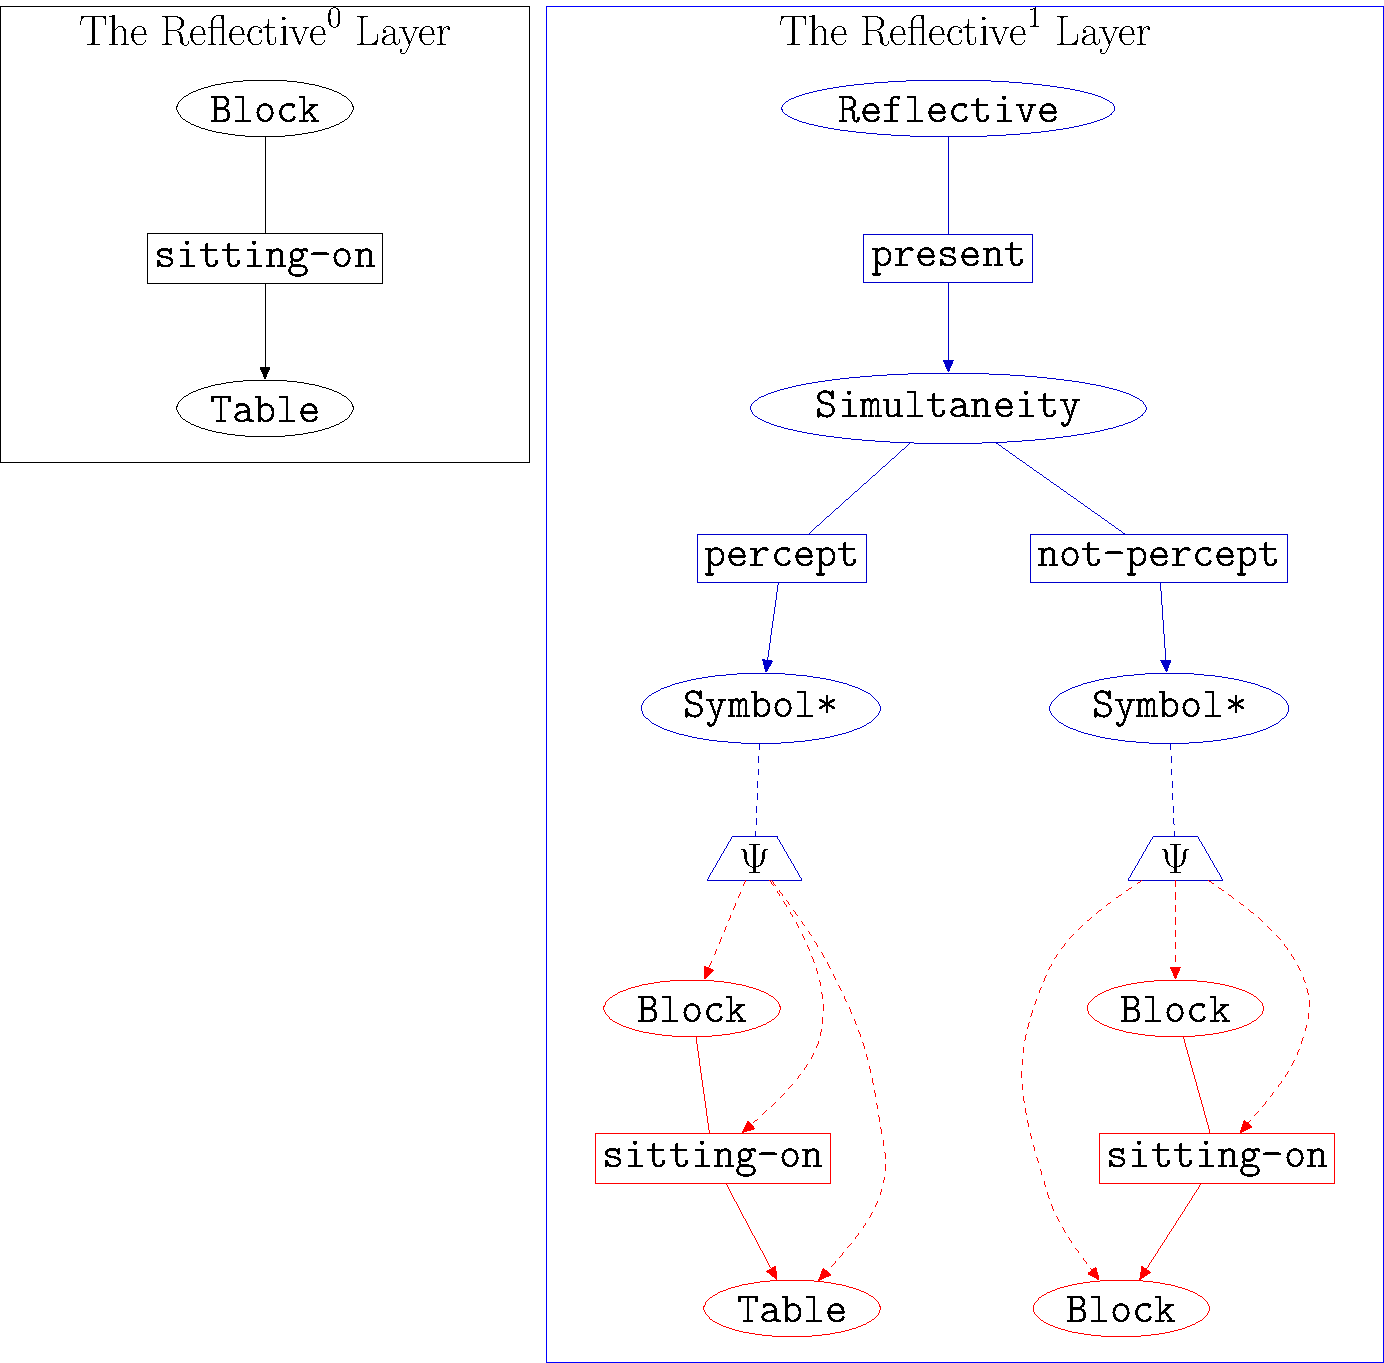
\includegraphics[width=10cm]{gfx/example_simultaneity}
\caption[Example simultaneity of positive and negative symbolic
  perceptions.]{Example simultaneity of positive and negative symbolic
  perceptions, where the symbolic reference to the dynamic physical
  activity of a block sitting on a table is perceived, while a block
  sitting on another block is not.}
\label{figure:example_simultaneity}
\end{figure}

\section{Transitions}

Simultaneities can be ordered in temporal relationships in each
reflective layer.
{\mbox{Equation~\ref{equation:define_reflective_n_time}}} defines the
graph representation in the simulation state, $S$, that keeps track of
the grounded knowledge of all temporal orderings of previous
perceptual simultaneities.
\begin{equation}
\label{equation:define_reflective_n_time}
\text{\tt{reflective}}^n.\text{\tt{time}} \equiv \text{\emph{Transitions of the $\text{Reflective}^n$ Layer}}
\end{equation}
Given this representation of temporal orderings for each
$\text{reflective}^n$ layer,
{\mbox{Equations~\ref{equation:reflective_n_temporal_ordering_first}}}
{\mbox{and~\ref{equation:reflective_n_temporal_ordering_last}}} define
the transitive temporal relationship, $\stackrel{n}{<}$, that
describes a separate ordering of grounded simultaneities for each
reflective layer.
\begin{align}
\label{equation:reflective_n_temporal_ordering_first}
\left(\begin{array}{l}
  x^* \in \text{\tt{reflective}}^n.\text{\tt{time}} ~\wedge~ \\
  ~~t_1^* \in x^*.\text{\tt{past}} ~\wedge~ t_2^* \in x^*.\text{\tt{future}}
\end{array}\right) &\longrightarrow t_1 \stackrel{n}{<} t_2 \\
\label{equation:reflective_n_temporal_ordering_last}
(t_1 \stackrel{n}{<} t_2 ~\wedge~ t_2 \stackrel{n}{<} t_3) &\longrightarrow t_1 \stackrel{n}{<} t_3
\end{align}
{\mbox{Equation~\ref{equation:reflective_n_temporally_ordered_set}}}
defines the separate set of ordered simultaneities within each
$\text{reflective}^n$ layer.
\begin{equation}
\label{equation:reflective_n_temporally_ordered_set}
 T^{n*} = \left\{t^* : 
\begin{array}{l}
  x^* \in \text{\tt{reflective}}^n.\text{\tt{time}} ~\wedge~ \\
  ~~(t^* \in x^*.\text{\tt{past}} ~\vee~ t^* \in x^*.\text{\tt{future}})
\end{array}\right\}
\end{equation}
{\mbox{Equation~\ref{equation:define_time_connected_full_ordering}}}
defines each set of temporally ordered simultaneities, $T^{n*}$, is a
connected and fully ordered sequence.
\begin{equation}
\label{equation:define_time_connected_full_ordering}
(t^*_1 \in T^{n*} \wedge t^*_2 \in T^{n*}) \longrightarrow (t^*_1 \stackrel{n}{<} t^*_2 \vee t^*_2 \stackrel{n}{<} t^*_1 \vee t^*_1 = t^*_2)
\end{equation}
{\mbox{\autoref{figure:example_transition}}} shows an example of how
three simultaneities can be represented in a simulation state graph as
temporally ordered using two transition relationships.
\begin{figure}
\center
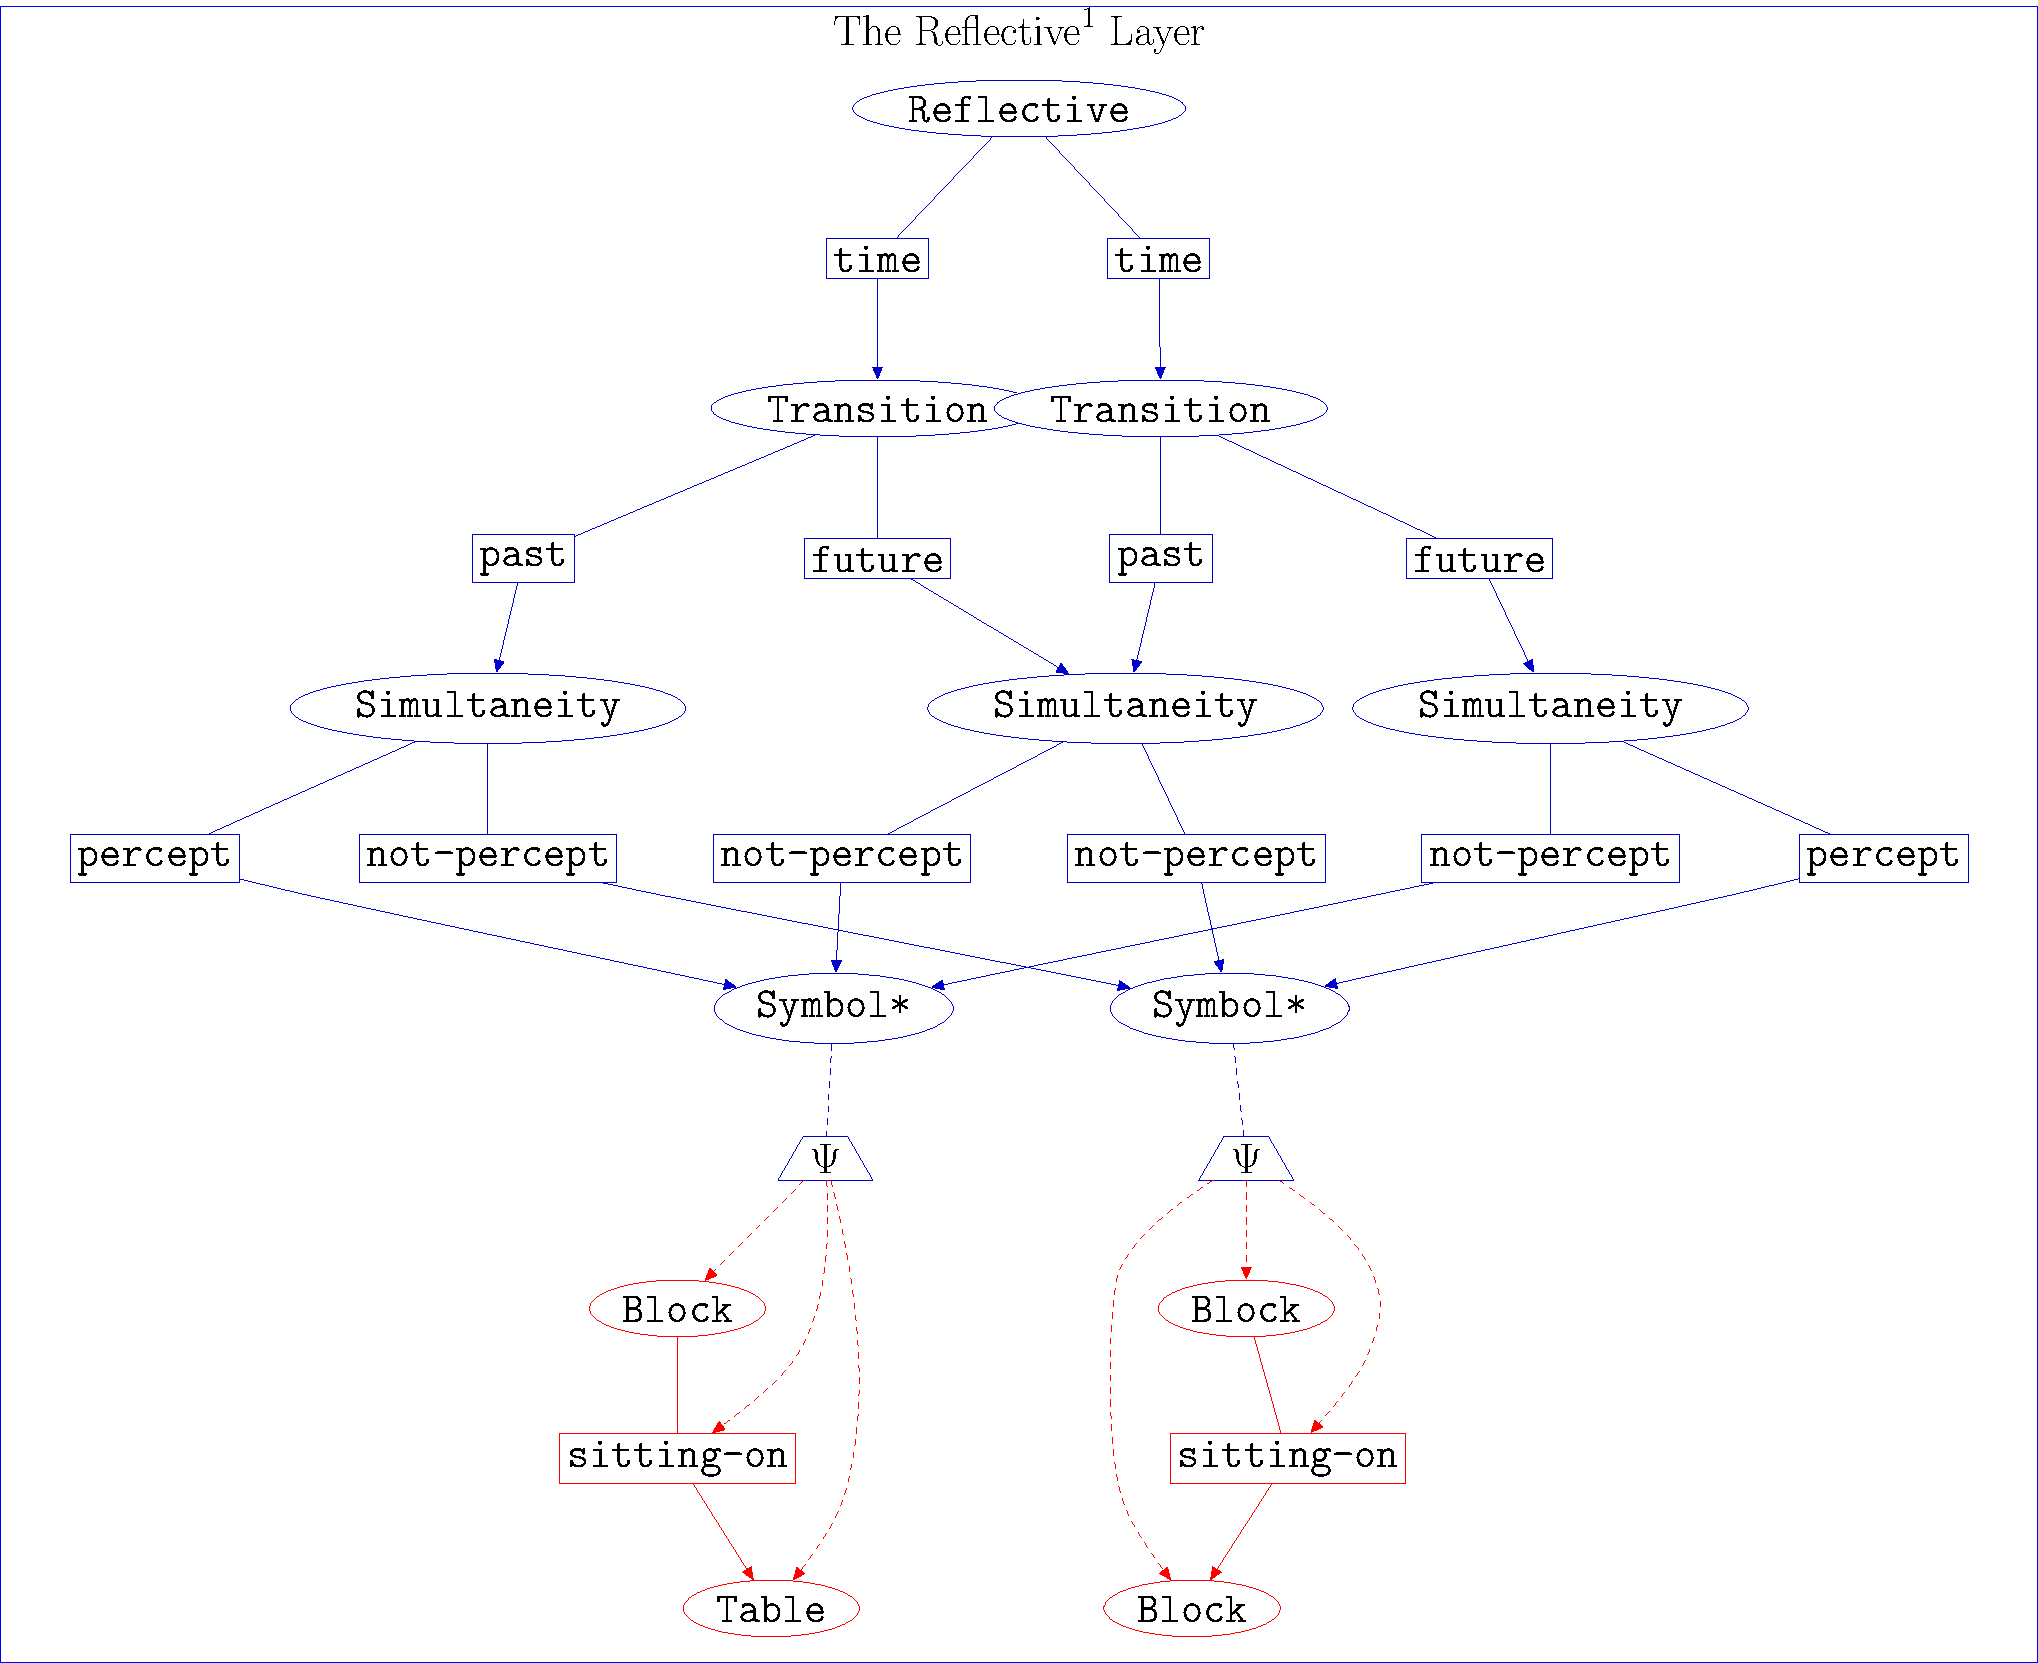
\includegraphics[width=14cm]{gfx/example_transition}
\caption[An example of two transitions ordering three
  simultaneities.]{An example of two transitions ordering three
  simultaneities: (1) a block sitting on a table, (2) a block not
  sitting on a table, and (3) a block sitting on another block.}
\label{figure:example_transition}
\end{figure}

\section{Perceptual Events}

{\mbox{Equation~\ref{equation:define_perceived}}} defines a
``perceived'' Spatial relationship for each reflective layer that can
exist between a temporal simultaneity, $t^*$, and a static symbolic
reference, $x^*$, to the layers below.
\begin{equation}
\label{equation:define_perceived}
\text{perceived}^n(t^*, x^*) = (t^* \in T^{n*} ~\wedge~ x^* \in t^*.\text{\tt{percept}})
\end{equation}
{\mbox{Equation~\ref{equation:define_event_start}}} defines the start
times for perceptual events in each reflective layer.  A perceptual
event begins at the time when a symbol is perceived and has just
immediately transitioned from not being perceived.
\begin{equation}
\label{equation:define_event_start}
\begin{array}{l}
  \text{start}^n(t^*, x^*) = \\
  ~~\left(
  \begin{array}{l}
  \text{perceived}^n(t^*, x^*) ~\wedge~ \\
  ~~\left[
  \begin{array}{l}
  \forall_{t_1^* \in T^{n*}}, \\
  ~~\left(\begin{array}{l}
            \left[\begin{array}{l}
                    t_1^* \stackrel{n}{<} t^* ~\wedge~ \\
                    ~~\text{perceived}^n(t_1^*, x^*)\end{array}\right] \longrightarrow \\
            ~~\exists_{t_2^* \in T^{n*}}, \\
            ~~~~\left[\begin{array}{l}
                        t_1^* \stackrel{n}{<} t_2^* \stackrel{n}{<} t^* ~\wedge~ \\
                        ~~\neg\text{perceived}^n(t_2^*, x^*)\end{array}\right]\end{array}\right)
  \end{array}
  \right]
  \end{array}\right)
\end{array}
\end{equation}
{\mbox{Equation~\ref{equation:define_event_end}}} defines the end
times for perceptual events in each reflective layer.  A perceptual
event ends at the time when a symbol is perceived and will immediately
transition to not being perceived at the subsequent time.
\begin{equation}
\label{equation:define_event_end}
\begin{array}{l}
  \text{end}^n(t^*, x^*) = \\
  ~~\left(
  \begin{array}{l}
  \text{perceived}^n(t^*, x^*) ~\wedge~ \\
  ~~\left[
  \begin{array}{l}
  \forall_{t_1^* \in T^{n*}}, \\
  ~~\left(\begin{array}{l}
            \left[\begin{array}{l}
                    t^* \stackrel{n}{<} t_1^* ~\wedge~ \\
                    ~~\text{perceived}^n(t_1^*, x^*)\end{array}\right] \longrightarrow \\
            ~~\exists_{t_2^* \in T^{n*}}, \\
            ~~~~\left[\begin{array}{l}
                        t^* \stackrel{n}{<} t_2^* \stackrel{n}{<} t_1^* ~\wedge~ \\
                        ~~\neg\text{perceived}^n(t_2^*, x^*)\end{array}\right]\end{array}\right)
  \end{array}
  \right]
  \end{array}\right)
\end{array}
\end{equation}
Between the start and end times of a perceptual event, a symbol has
been continuously perceived.  Event knowledge is factual knowledge
that is grounded in the perception of the dynamic.  Factual knowledge
does not involve hypothetical reasoning.  Later, I will show how
hypothetical assumptions can be abstracted from factual event
knowledge.  Grounded factual knowledge is the source of all
hypothetical abstractions that are used in planning.  Thus, grounded
knowledge is the necessary foundation for creating a planning
algorithm that can be debugged when the hypothetical bases of
counterfactual knowledge turn out to be contradicted by further
factual knowledge.
{\mbox{Equations~\ref{equation:define_perceptual_event_first}}}
{\mbox{through~\ref{equation:define_perceptual_event_last}}} define a
perceptual event in the $n^{\text{th}}$-order reflective layer.
\begin{align}
\label{equation:define_perceptual_event_first}
                                         e^* &\in \text{\tt{reflective}}^n.\text{\tt{event}} \\
                      e^*.\text{\tt{symbol}} &= \{x^*\} \\
                       e^*.\text{\tt{start}} &= \{t^*_\text{start}\} \\
                         e^*.\text{\tt{end}} &= \{t^*_\text{end}\} \\
                             t^*_\text{start} &\in \{t^* : t^* \in T^{n*} \wedge \text{start}^n(t^*, x^*)\} \\
                               t^*_\text{end} &\in \{t^* : t^* \in T^{n*} \wedge \text{end}^n(t^*, x^*)\} \\
                             t^*_\text{start} &\stackrel{n}{<} t^*_\text{end} \\
\label{equation:define_perceptual_event_last}
 \neg\exists_{t^* \in T^{n*}}, [t^*_\text{start} &\stackrel{n}{<} t^* \stackrel{n}{<} t^*_\text{end} \wedge \text{end}^n(t^*, x^*)]
\end{align}

\section{Event Transframes}

While transitions represent a temporal relationship between two
simultaneities, a \emph{transframe} represents the difference between
two simultaneities.  For example, two simultaneities could both
contain a lot of perceptual information, but the transframe between
them might be a very small set of differences.  The difference between
two simultaneities is kept track of as two lists: (1) the additions
and (2) the removals from the actively perceived symbols in each
simultaneity.  {\mbox{\autoref{figure:example_transframe}}} shows an
example of a perceptual event that has an associated transframe.
\begin{figure}
\center
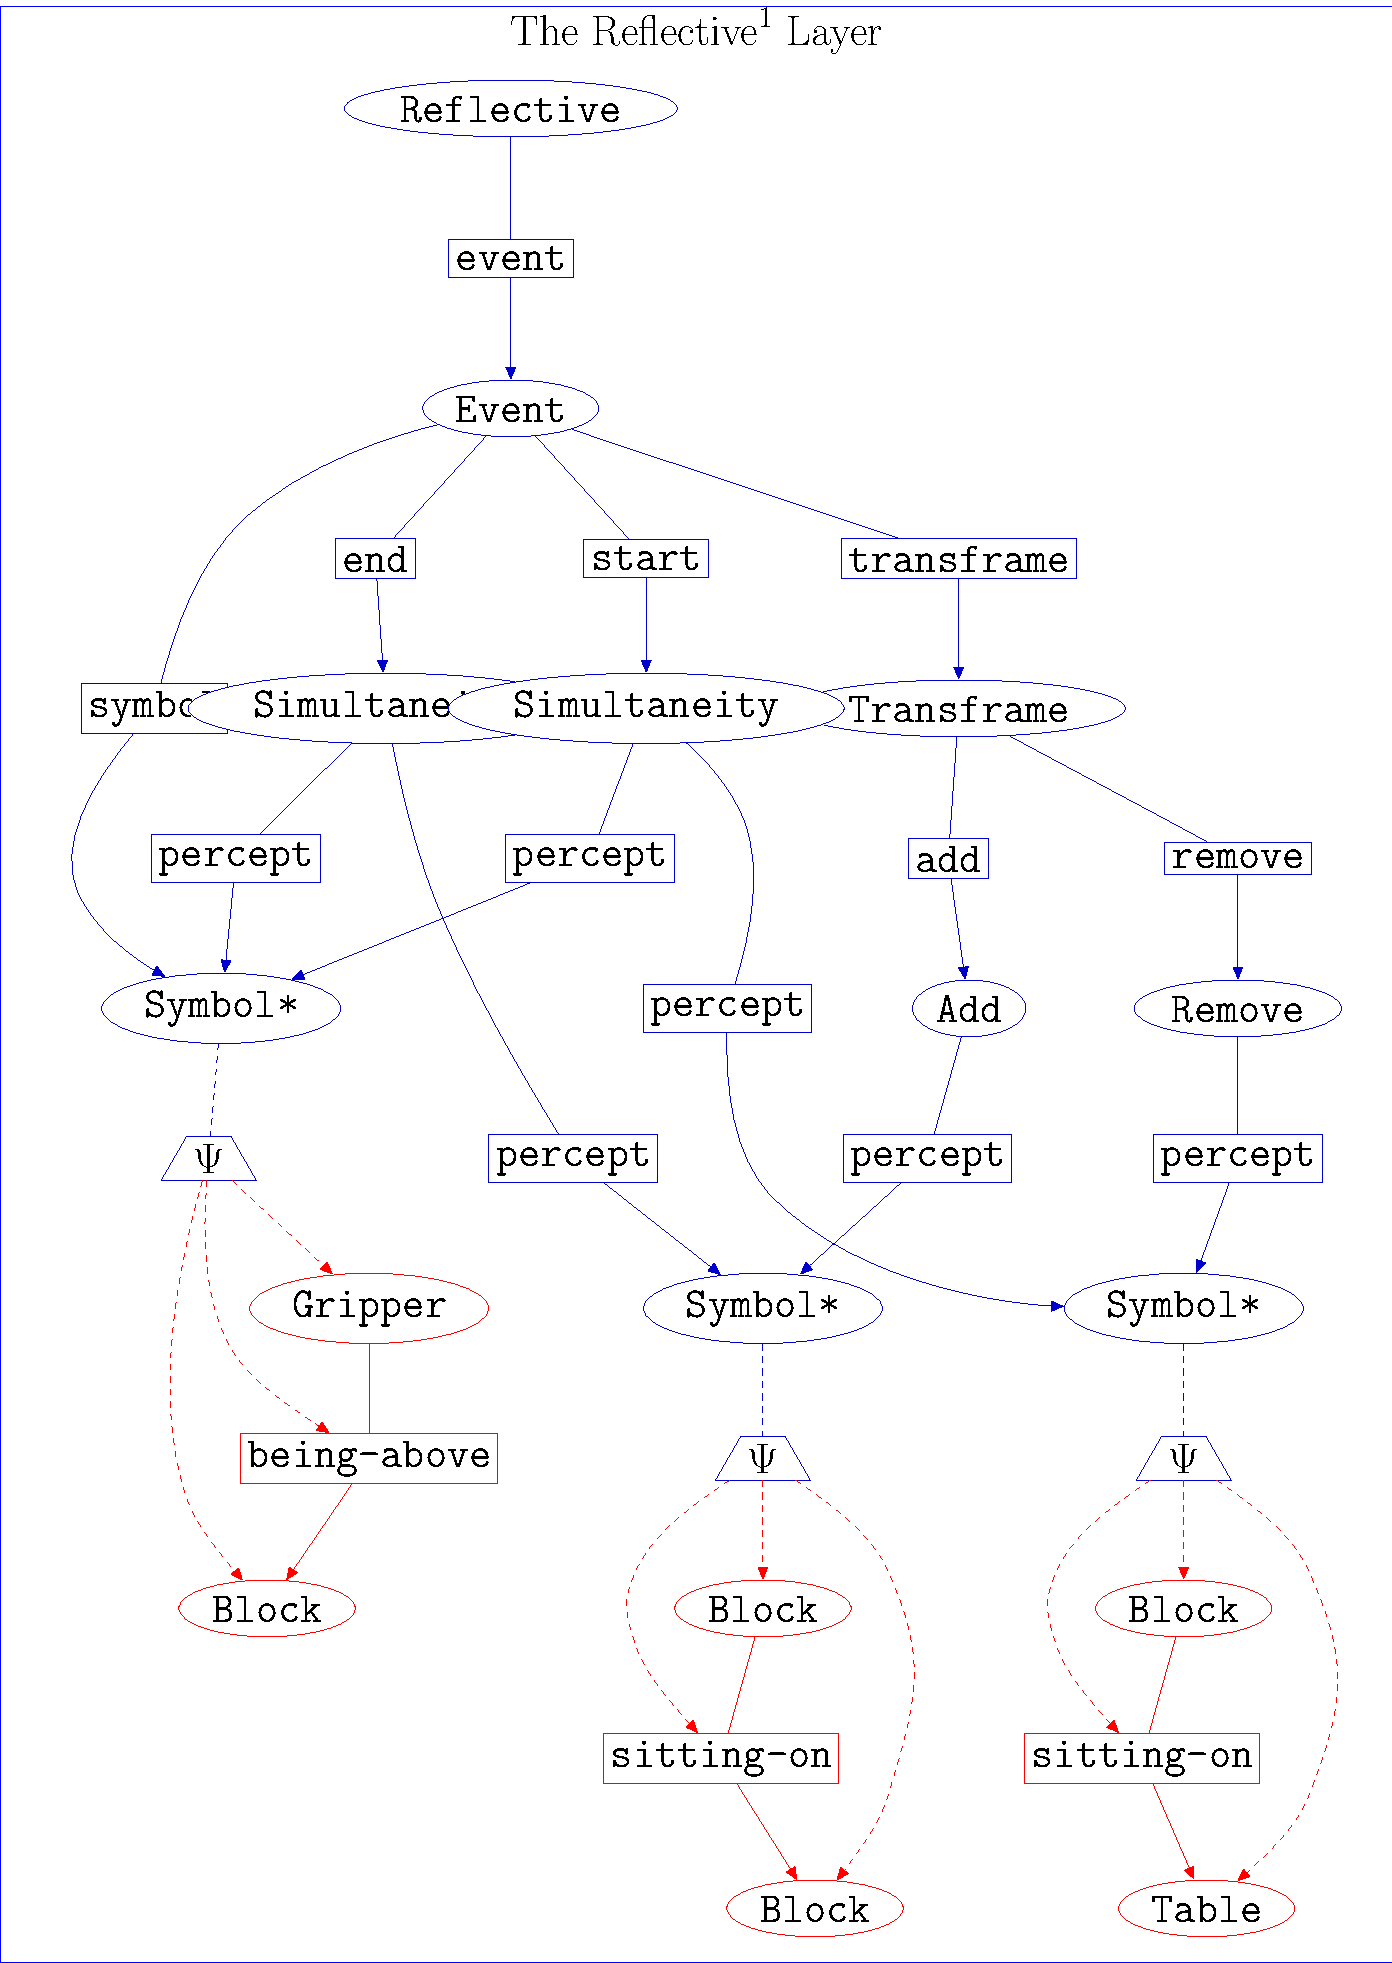
\includegraphics[width=12cm]{gfx/example_transframe}
\caption[An example of a factual event transframe.]{An example of a
  factual event transframe, representing the continuous perception of
  the symbol that refers to the dynamic physical activity of a gripper
  being above a block.  The symbolized perceptual difference between
  the starting and ending simultaneities is represented by a
  transframe of the perceptual event, listing the symbolic additions
  and removals from the starting and ending situations.  Note that
  negative perceptions in both the simultaneities and the transframe
  have been omitted for clarity.}
\label{figure:example_transframe}
\end{figure}

\section{Action Resources}

{\mbox{\autoref{figure:example_resource}}} shows an example of a
resource in the first-order reflective thinking layer.
\begin{figure}
\center
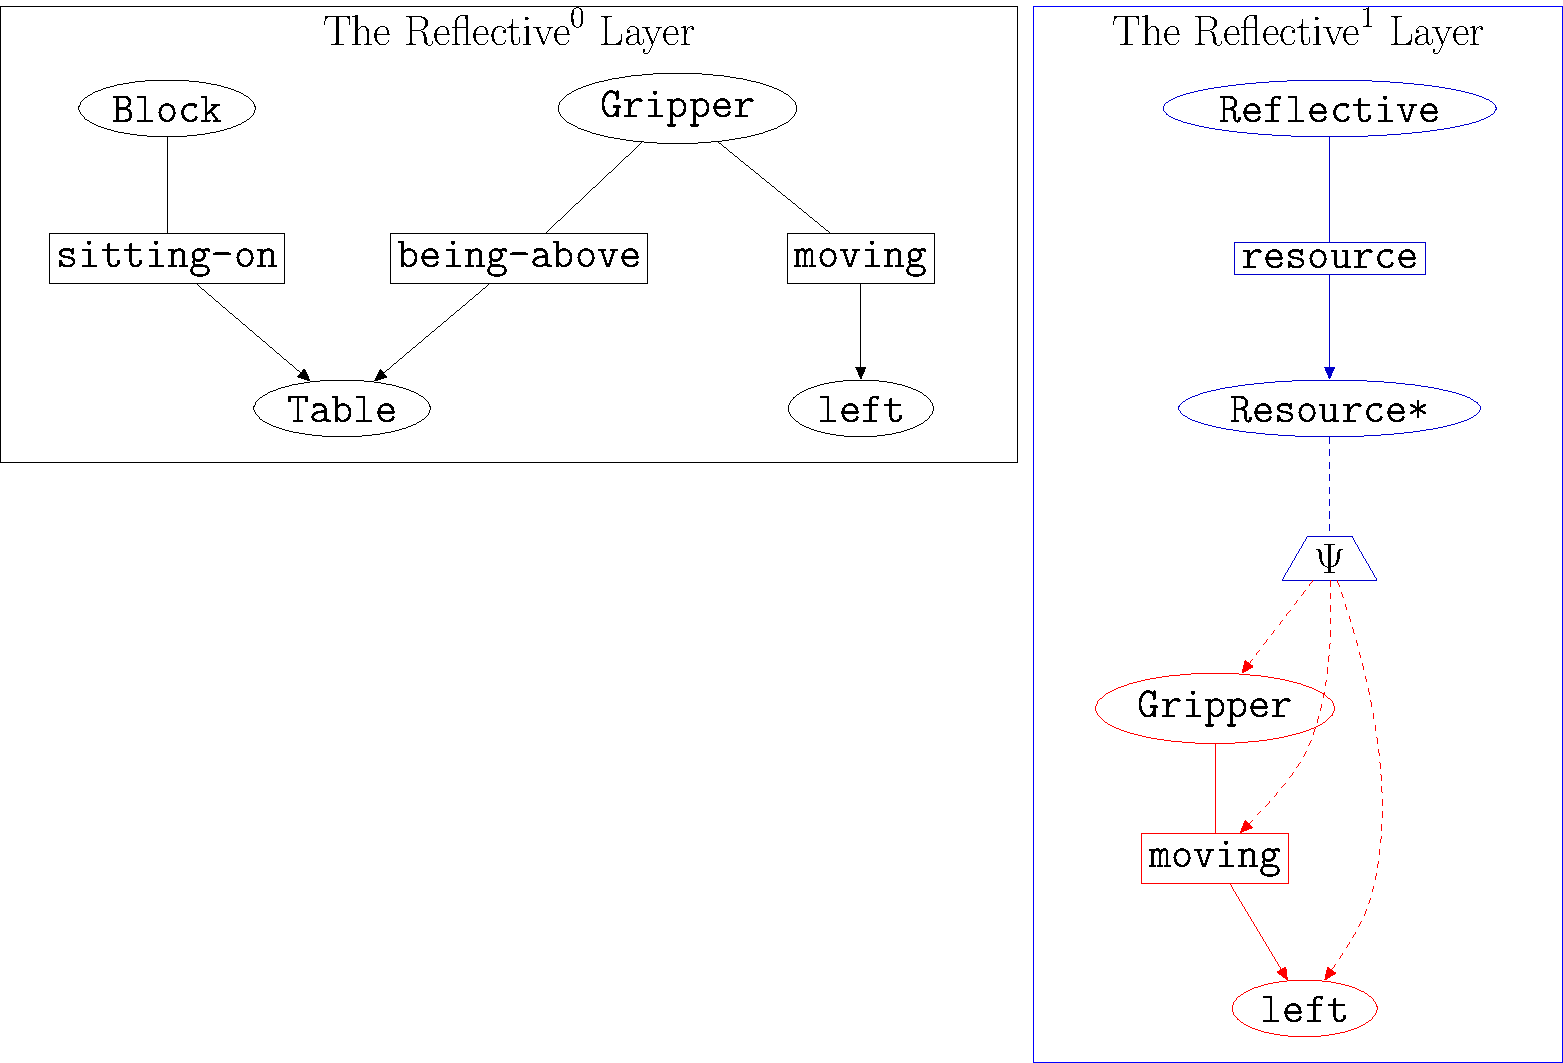
\includegraphics[width=6cm]{gfx/example_resource}
\caption{An example of a first-order reflective resource.}
\label{figure:example_resource}
\end{figure}




\section{leftovers...}

\section{Causal Knowledge}

Now that a separate temporal sequence for each reflective layer has
been defined, this factual grounded knowledge can be abstracted into
hypothetical causal models that are useful for planning toward goals
in a counterfactual future.



{\mbox{\autoref{figure:example_causal_knowledge}}} shows an example of
causal knowledge.
\begin{figure}
\center
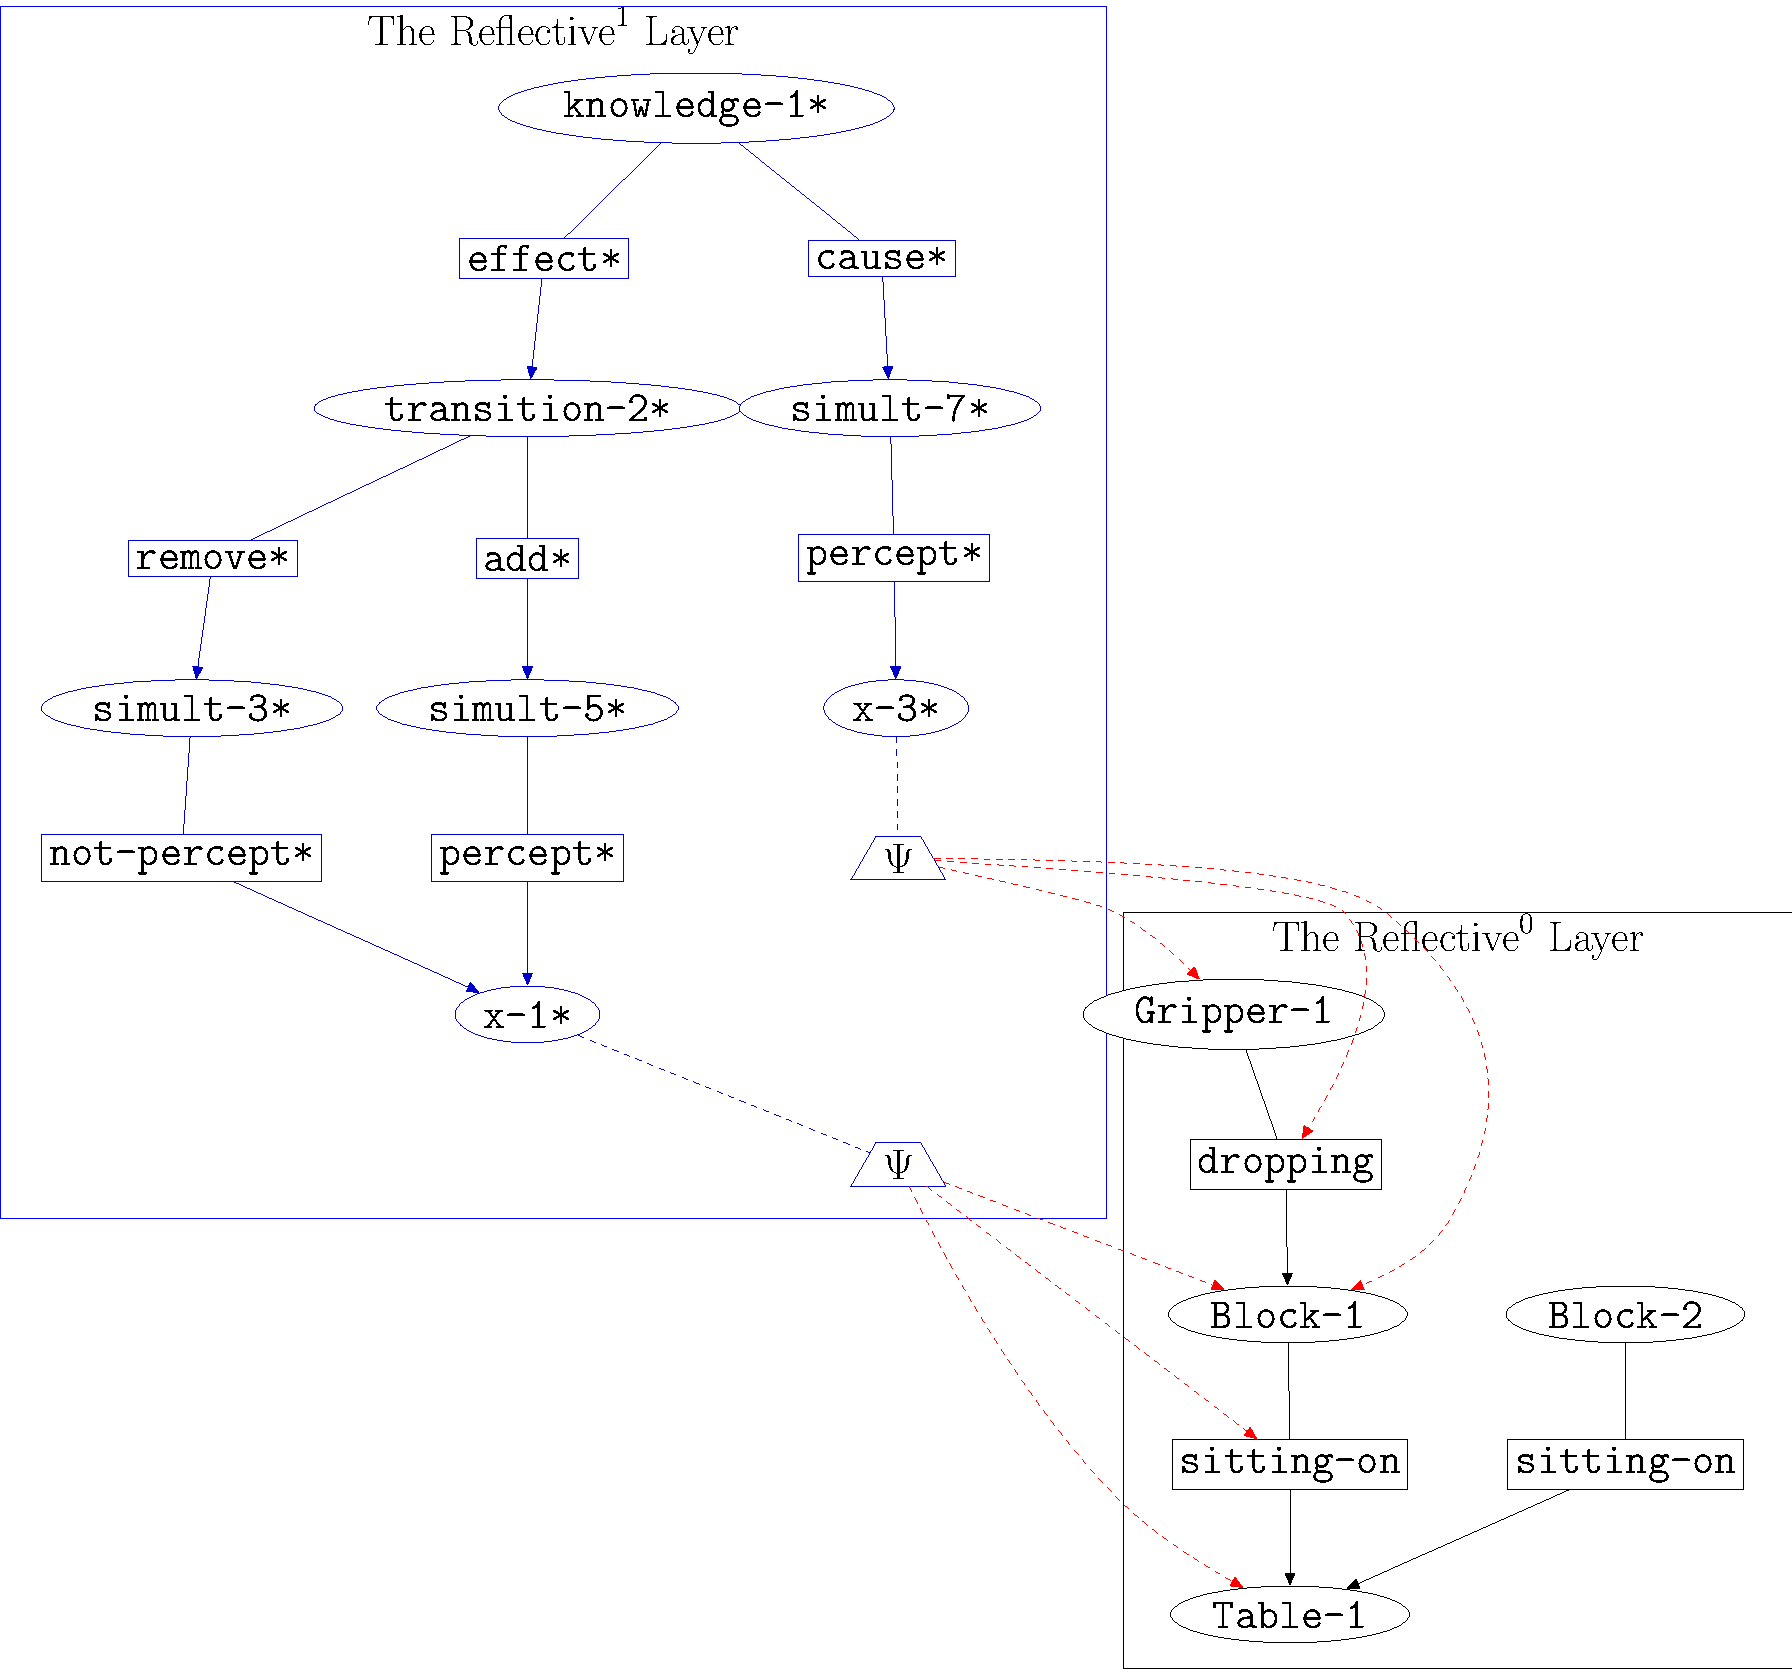
\includegraphics[width=12cm]{gfx/example_causal_knowledge}
\caption[An example of a causal knowledge.]{An example of causal
  knowledge, $\text{\tt{knowledge}}_1^*$, where the simultaneity,
  $\text{\tt{simult}}_7^*$, is known to be the cause of the
  transframe, $\text{\tt{transition}}_2^*$.  Negative perceptions are
  omitted here for to reduce visual clutter.}
\label{figure:example_causal_knowledge}
\end{figure}

\section{Representing Causal Hypotheses}

{\mbox{\autoref{figure:example_causal_hypothesis}}} shows an example
of a causal hypothesis, $h_1^*$, where the simultaneity,
$\text{\tt{simult}}_7^*$, is hypothesized to be the cause of the
transframe, $\text{\tt{transframe}}_2^*$.  In other words, the gripper
dropping the block causes the block to be sitting on the table.
\begin{figure}
\center
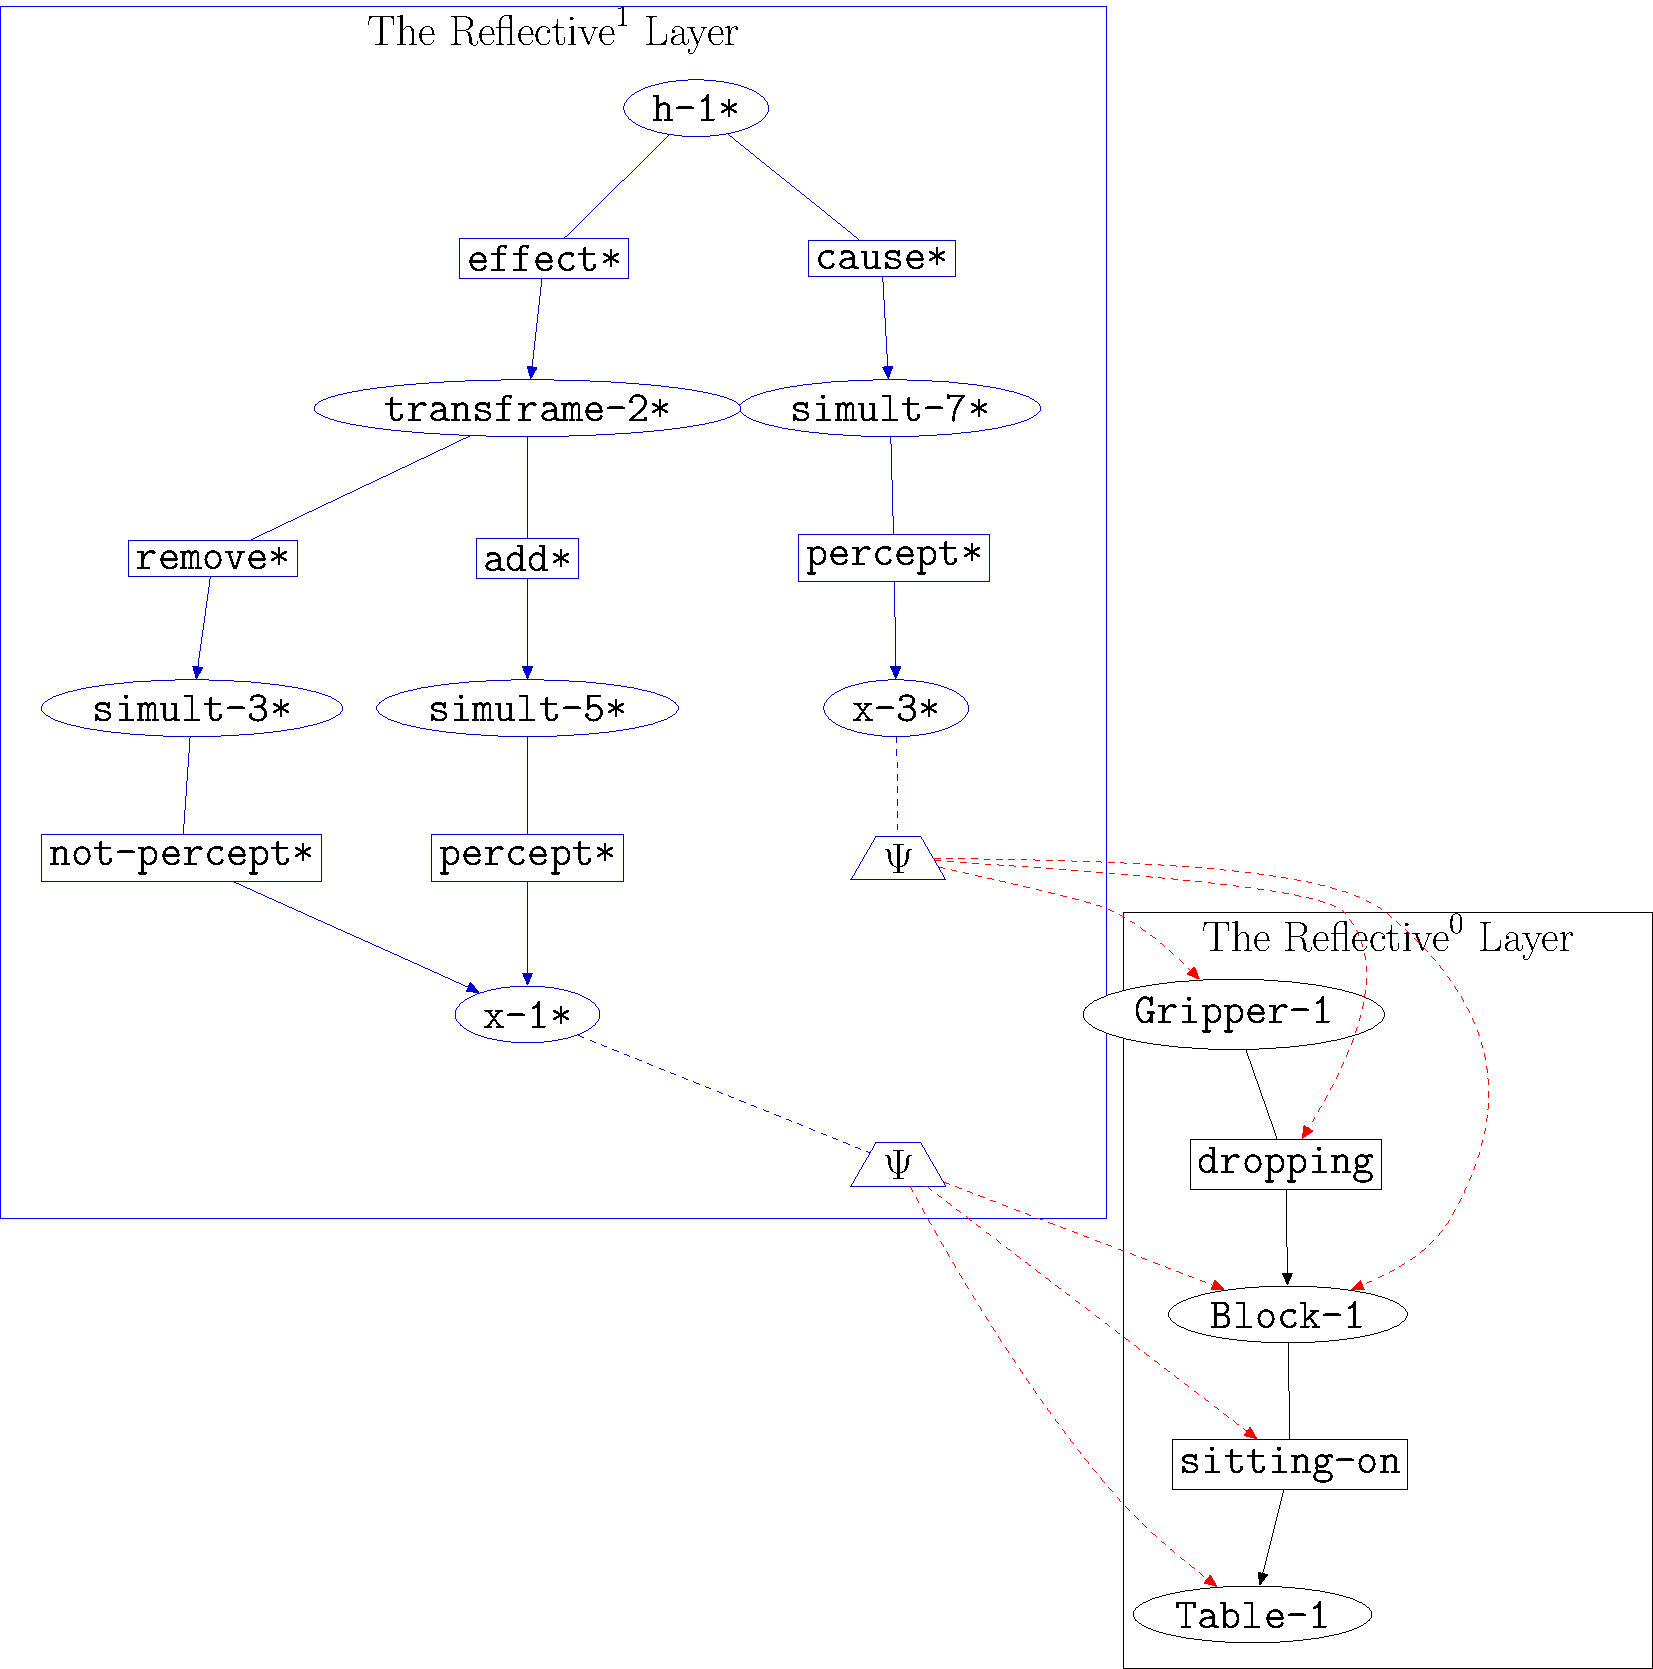
\includegraphics[width=8cm]{gfx/example_causal_hypothesis}
\caption[An example of a causal hypothesis.]{An example of a causal
  hypothesis, $h_1^*$, where the simultaneity,
  $\text{\tt{simult}}_7^*$, is hypothesized to be the cause of the
  transframe, $\text{\tt{transframe}}_2^*$.  In other words, the
  gripper dropping the block causes the block to be sitting on the
  table.}
\label{figure:example_causal_hypothesis}
\end{figure}

\section{Composing Plans from Hypotheses}

